% Section 4.5:
\subsection{Matriz de Consistencia}

\lipsum[17]

\lipsum[18]

\begin{figure}[!ht]
  \caption[Cuadro y gráficos que muestran el método N5]{Cuadro y gráficos que muestran el método N5. Adaptado de \cite{deWaal2009}}
  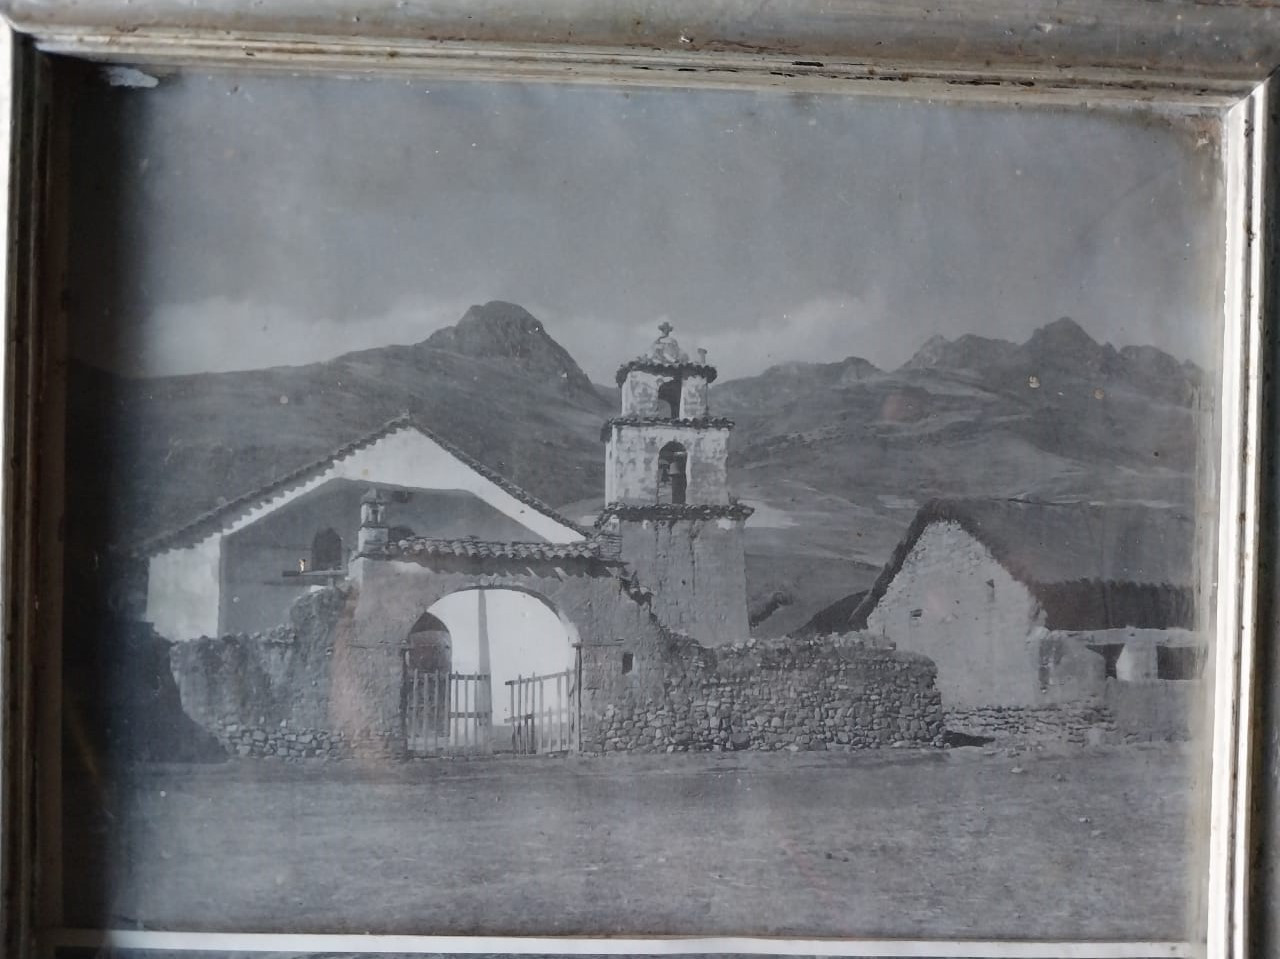
\includegraphics[scale=0.36]{F_Figures/15_Chapter VI/Cap6_Imagen1.jpeg}
  \figurenote{This is a great figure.}
	\label{Cap3_Figura3}
\end{figure}

\lipsum[22] en la Ecuación~\ref{equation124}


\begin{equation}\label{equation124}
  K_{i+1}=K_{i}+\frac{\left ( \delta g_{i}-K_{i}\delta u_{i} \right )c^{T}+c\left ( \delta g_{i}-K_{i}\delta u_{i} \right )^{T}}{c^{T}\delta u_i}-\frac{\left ( \delta g_{i}-K_{i}\delta u_{i} \right )^{T}\delta u_{i} c c^{T}}{\left ( c^{T}\delta u_{i} \right )^{2}}
\end{equation}
\myequations{Ecuación de Emin}